\documentclass[12pt]{article}
\usepackage{graphicx}
\usepackage{float}
\usepackage[margin=1in]{geometry}
\usepackage{setspace}
\usepackage{titlesec}

\setstretch{1.15}
\titleformat{\section}{\large\bfseries}{\thesection}{1em}{}

\title{A2: Cognitive Analysis \\ 48oz Nalgene Water Bottle}
\author{Alejandro De La Torre}
\date{}

\begin{document}
\maketitle

\section*{System Overview}

This analysis examines the interaction involved in refilling and securing a 48oz Nalgene water bottle using a Brita filter and kitchen sink. The selected task includes opening the bottle, filling it, evaluating when it is full, closing it securely, and transporting it.

The bottle is large, transparent, and uses a threaded screw-top lid with a plastic loop attachment. While simple, the system involves multiple cognitive judgments involving force, alignment, sensory feedback, and physical constraints.

\begin{figure}[H]
\centering
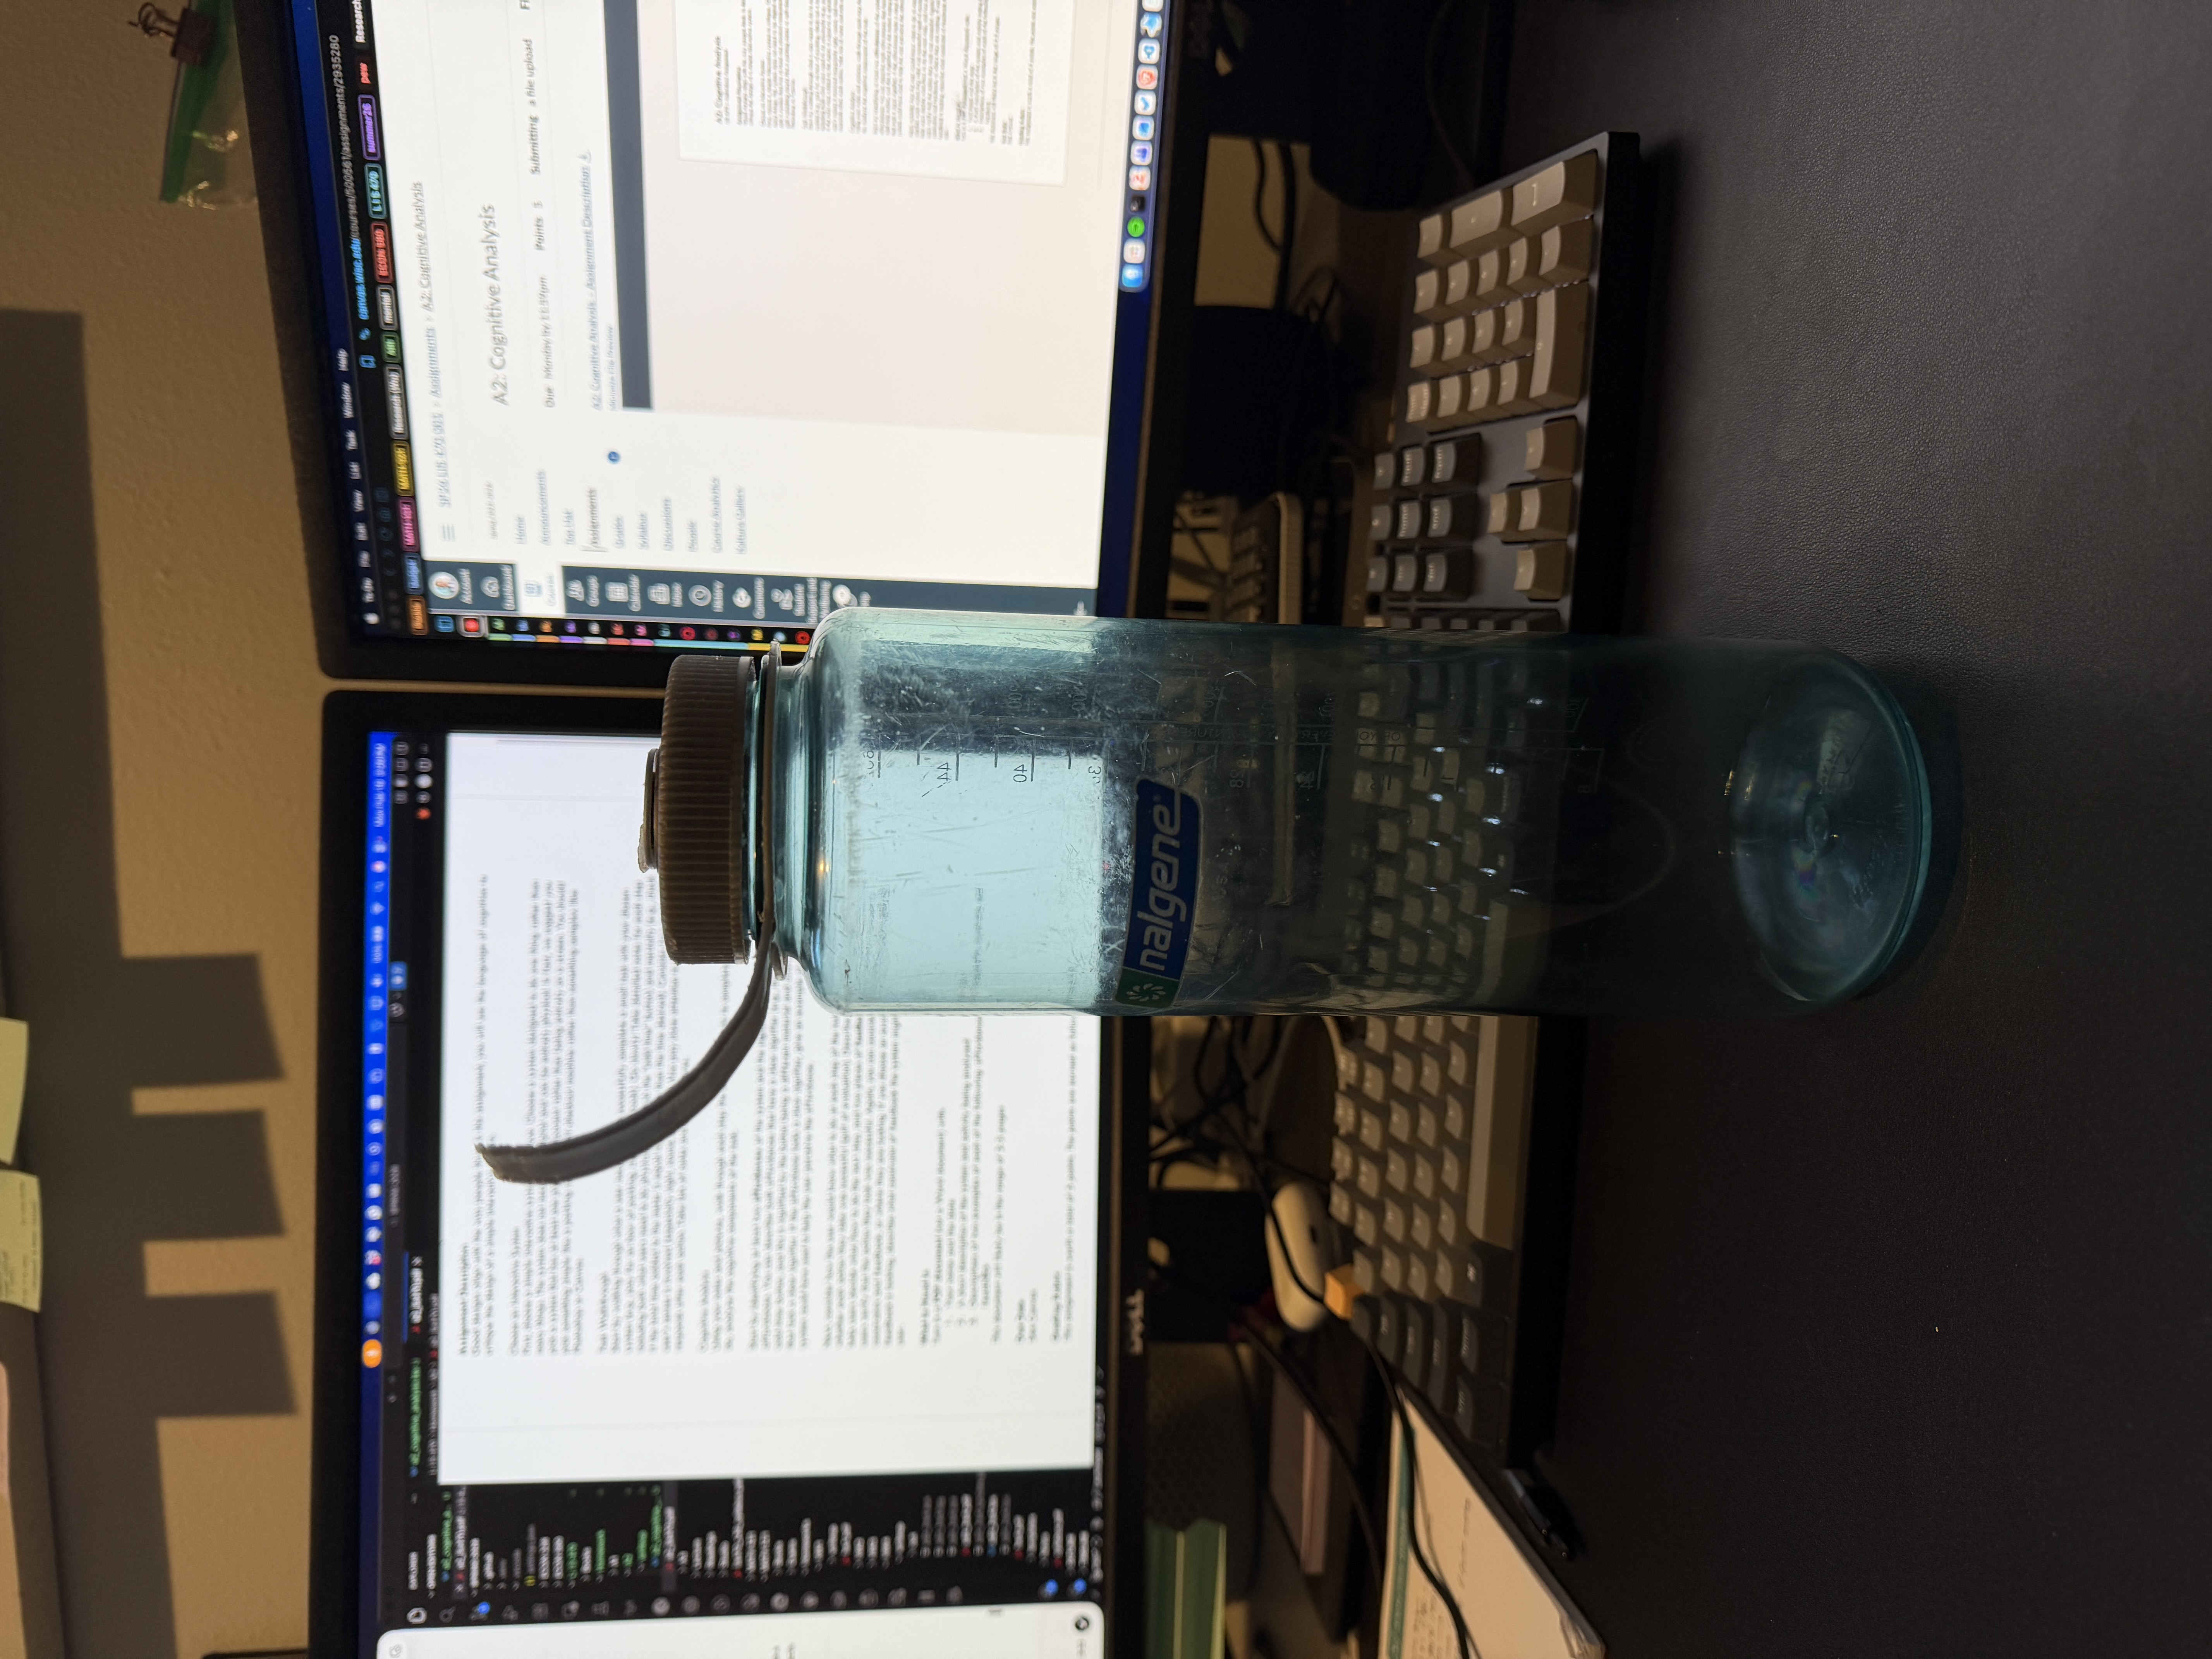
\includegraphics[width=0.45\textwidth,angle=-90]{images/bottle_on_desk.JPG}
\caption{48oz Nalgene bottle in resting state.}
\end{figure}

\section*{Task Walkthrough}

\subsection*{Step 1: Unscrewing the Lid}

The bottle is stabilized with one hand while the other twists the lid counterclockwise. The ridged texture on the lid supports grip and suggests rotational movement.

\begin{figure}[H]
\centering
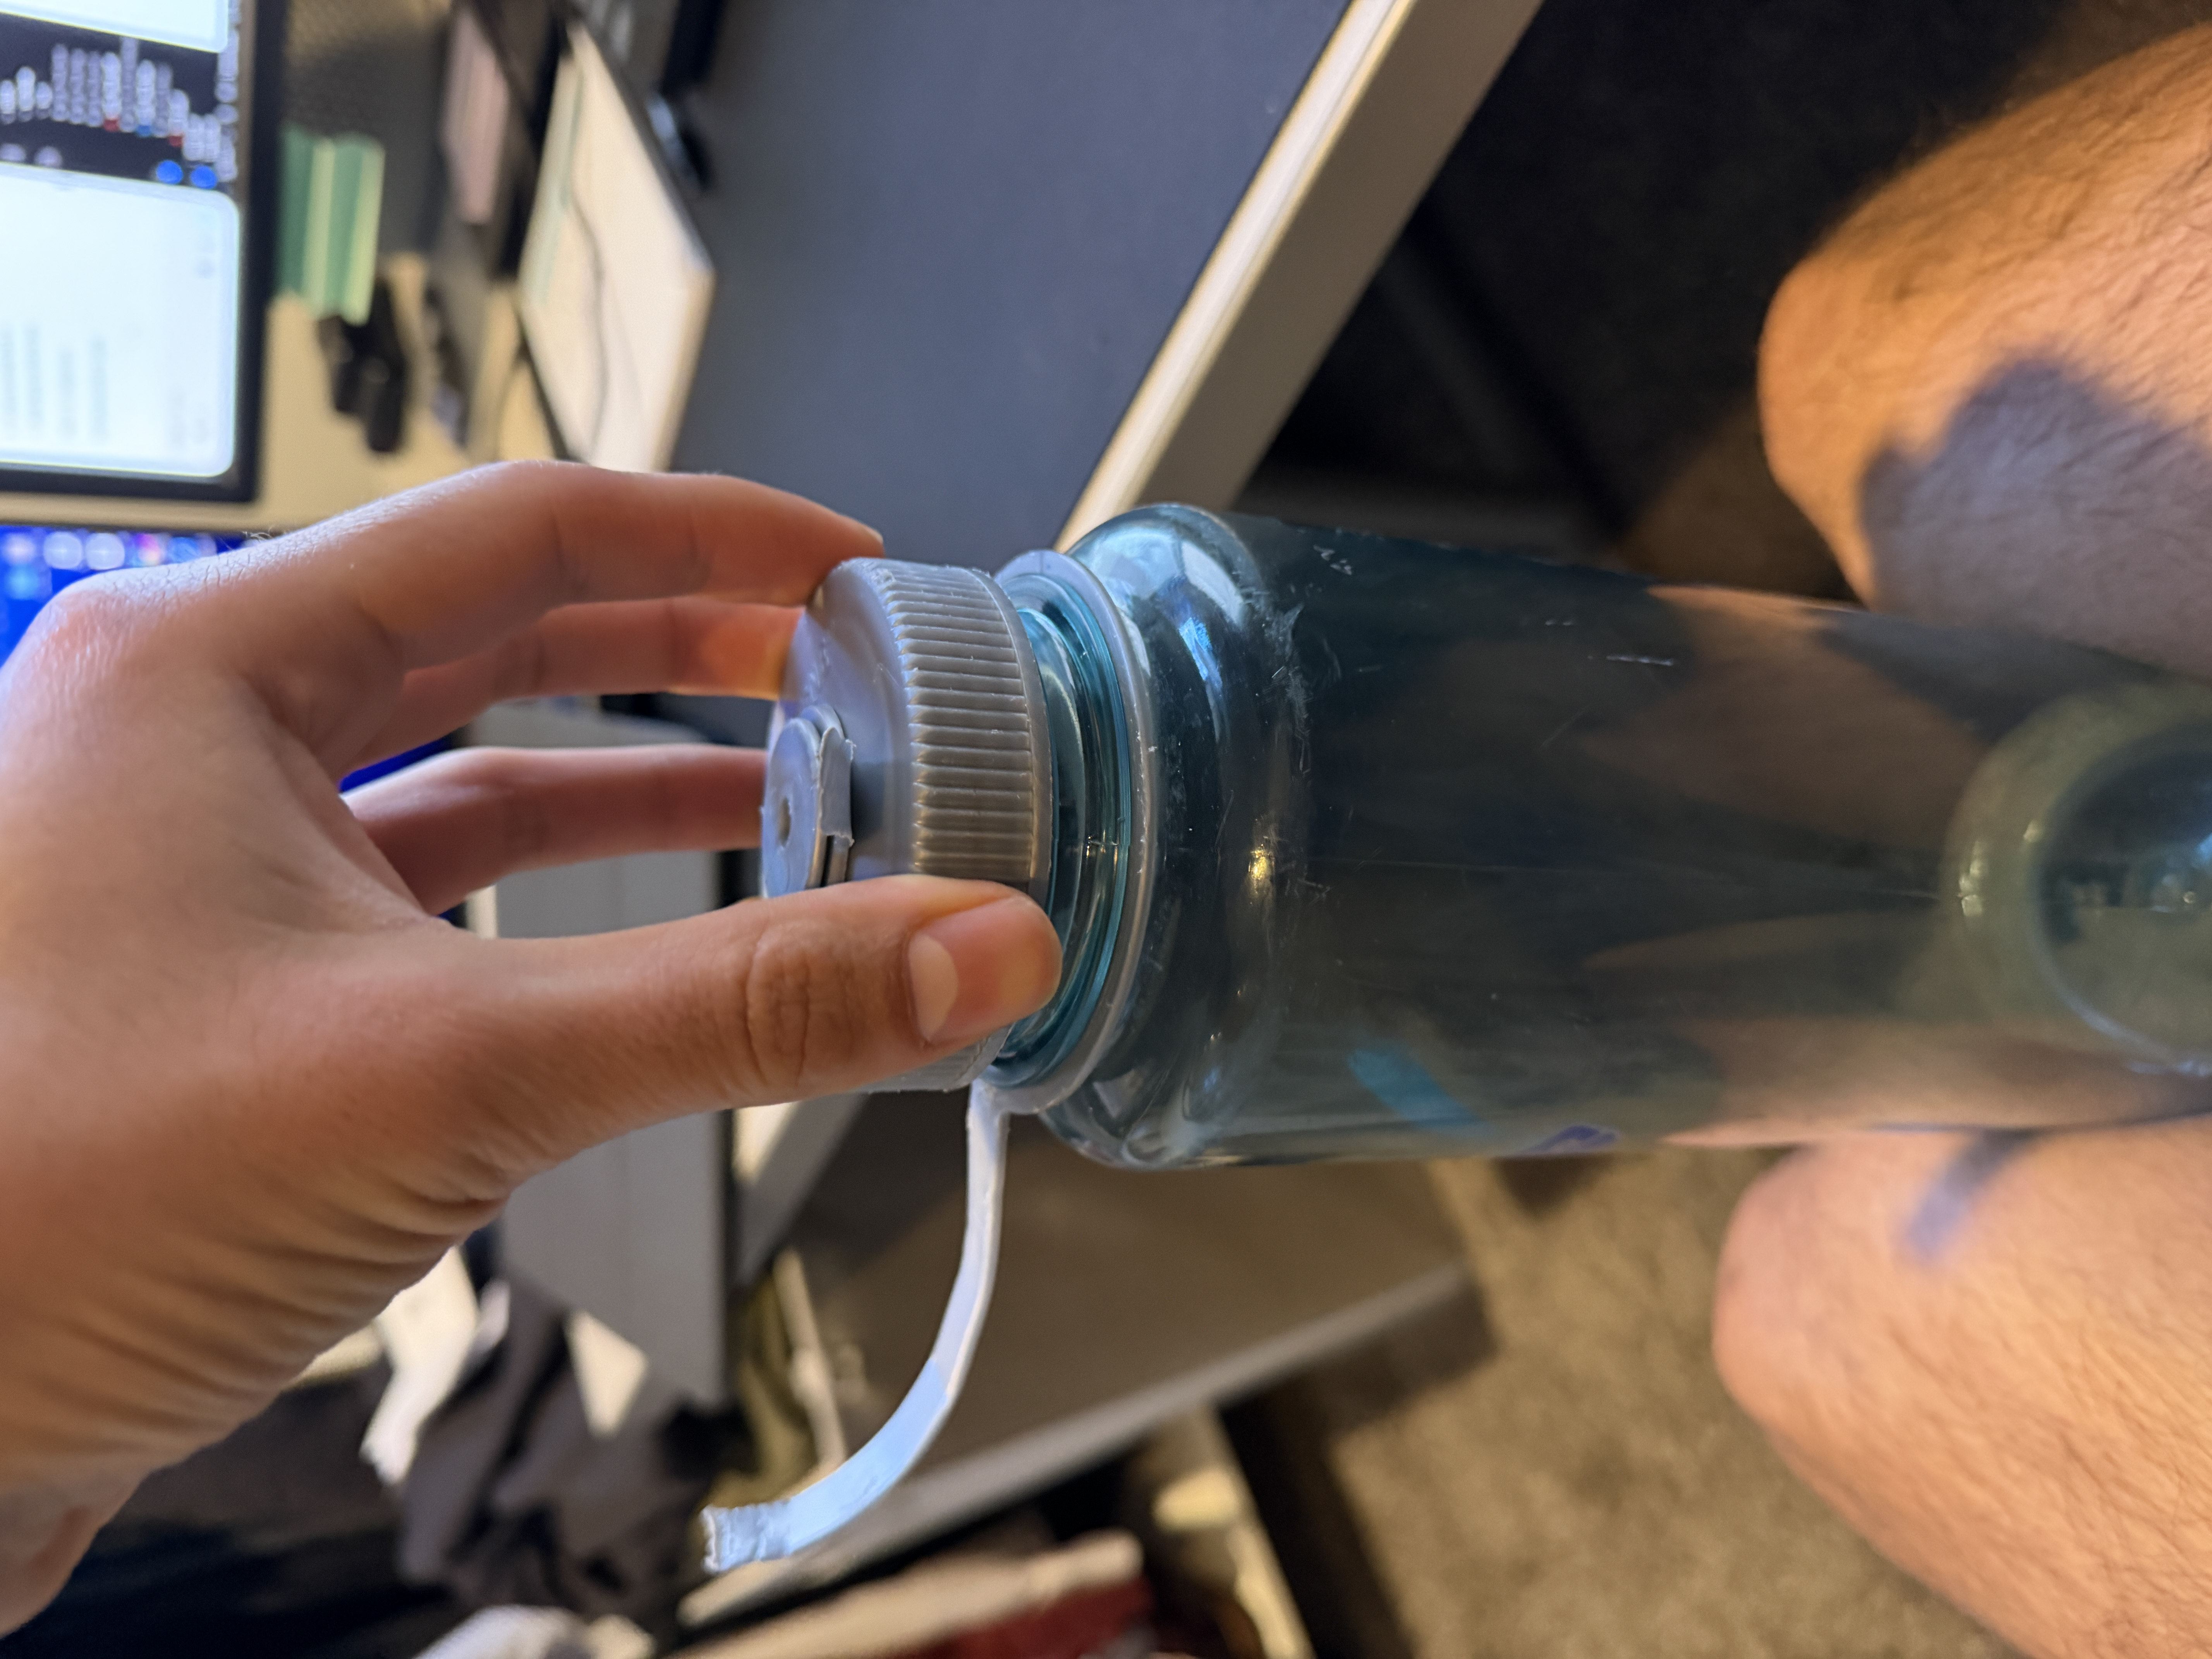
\includegraphics[width=0.45\textwidth,angle=-90]{images/hand-unscrewing-lid.JPG}
\caption{Two-handed interaction to unscrew lid.}
\end{figure}

The user relies on tactile feedback (decreasing resistance) and visible thread separation to know when the lid is disengaged.

\begin{figure}[H]
\centering
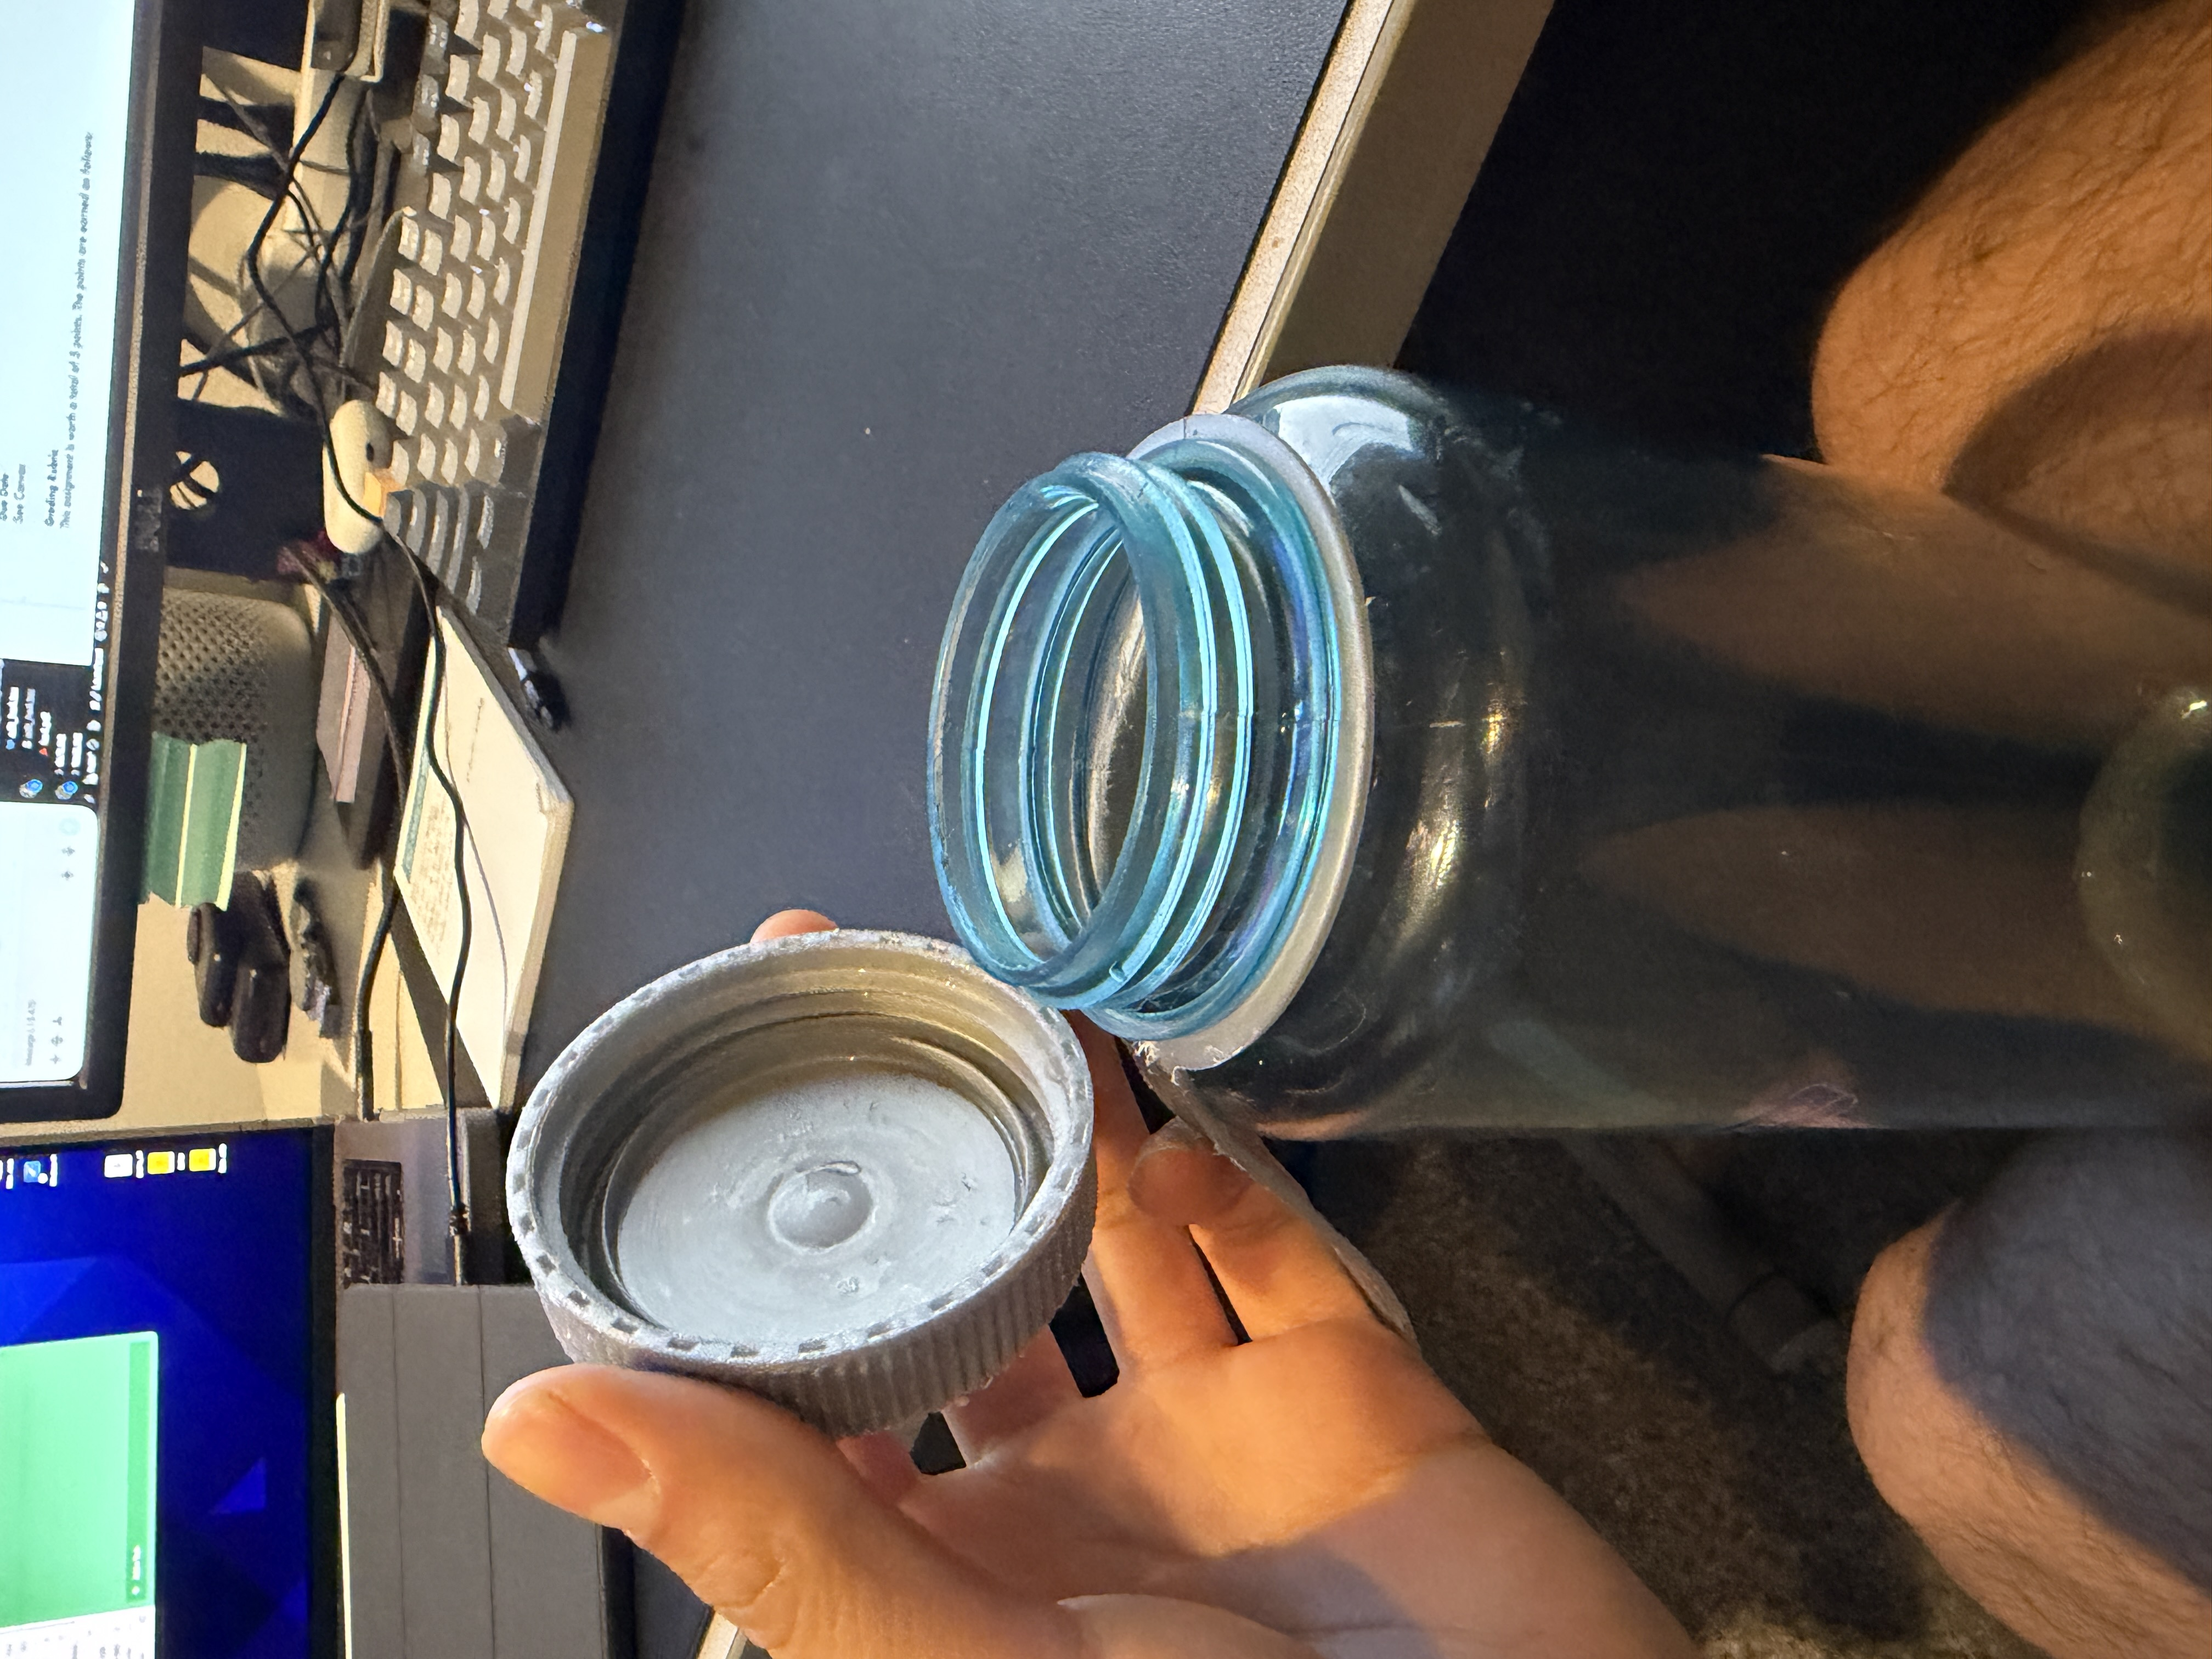
\includegraphics[width=0.45\textwidth,angle=-90]{images/lid-off-threads-visible.JPG}
\caption{Lid removed, threads visible.}
\end{figure}

\subsection*{Step 2: Filling the Bottle}

The bottle is positioned beneath the faucet. The wide opening affords direct filling. The user visually monitors rising water and listens to acoustic changes.

\begin{figure}[H]
\centering
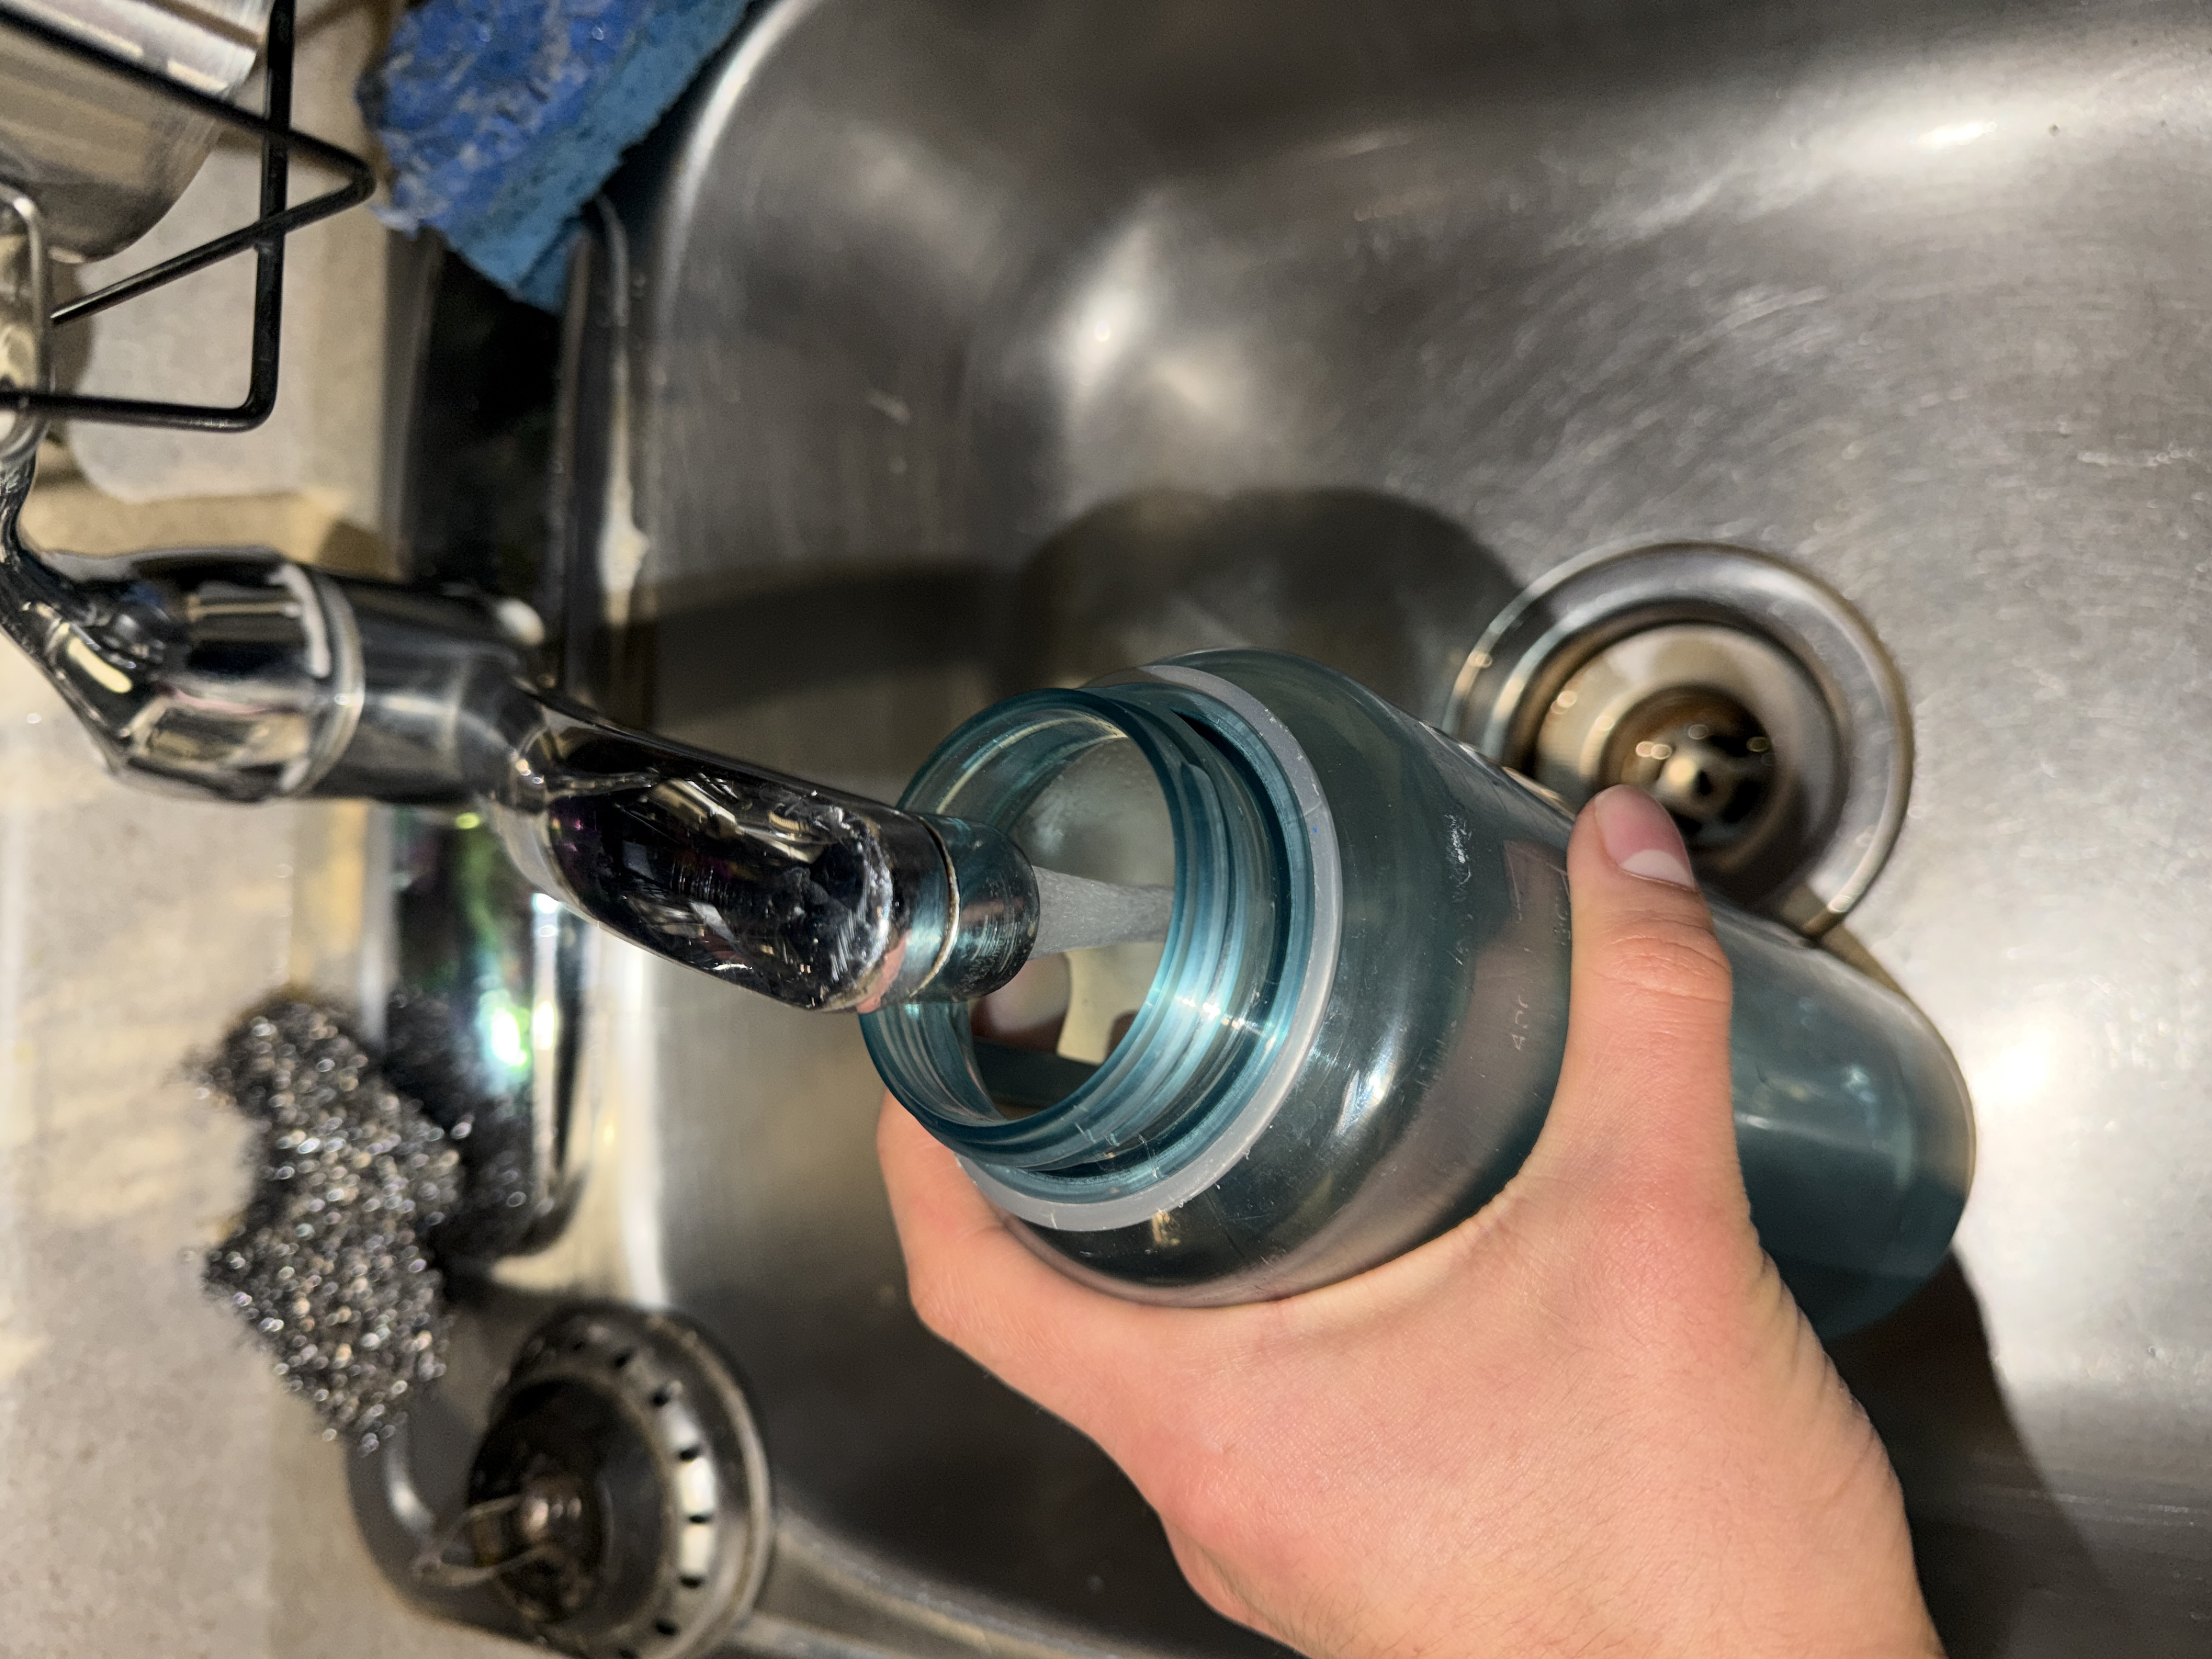
\includegraphics[width=0.45\textwidth,angle=-90]{images/bottle-under-faucet-filling.JPG}
\caption{Bottle positioned under faucet.}
\end{figure}

Stopping is determined primarily through:
\begin{itemize}
\item Visible bubbles reaching the top
\item Reduced echoing sound as air space decreases
\item Visible water line near rim
\end{itemize}

\begin{figure}[H]
\centering
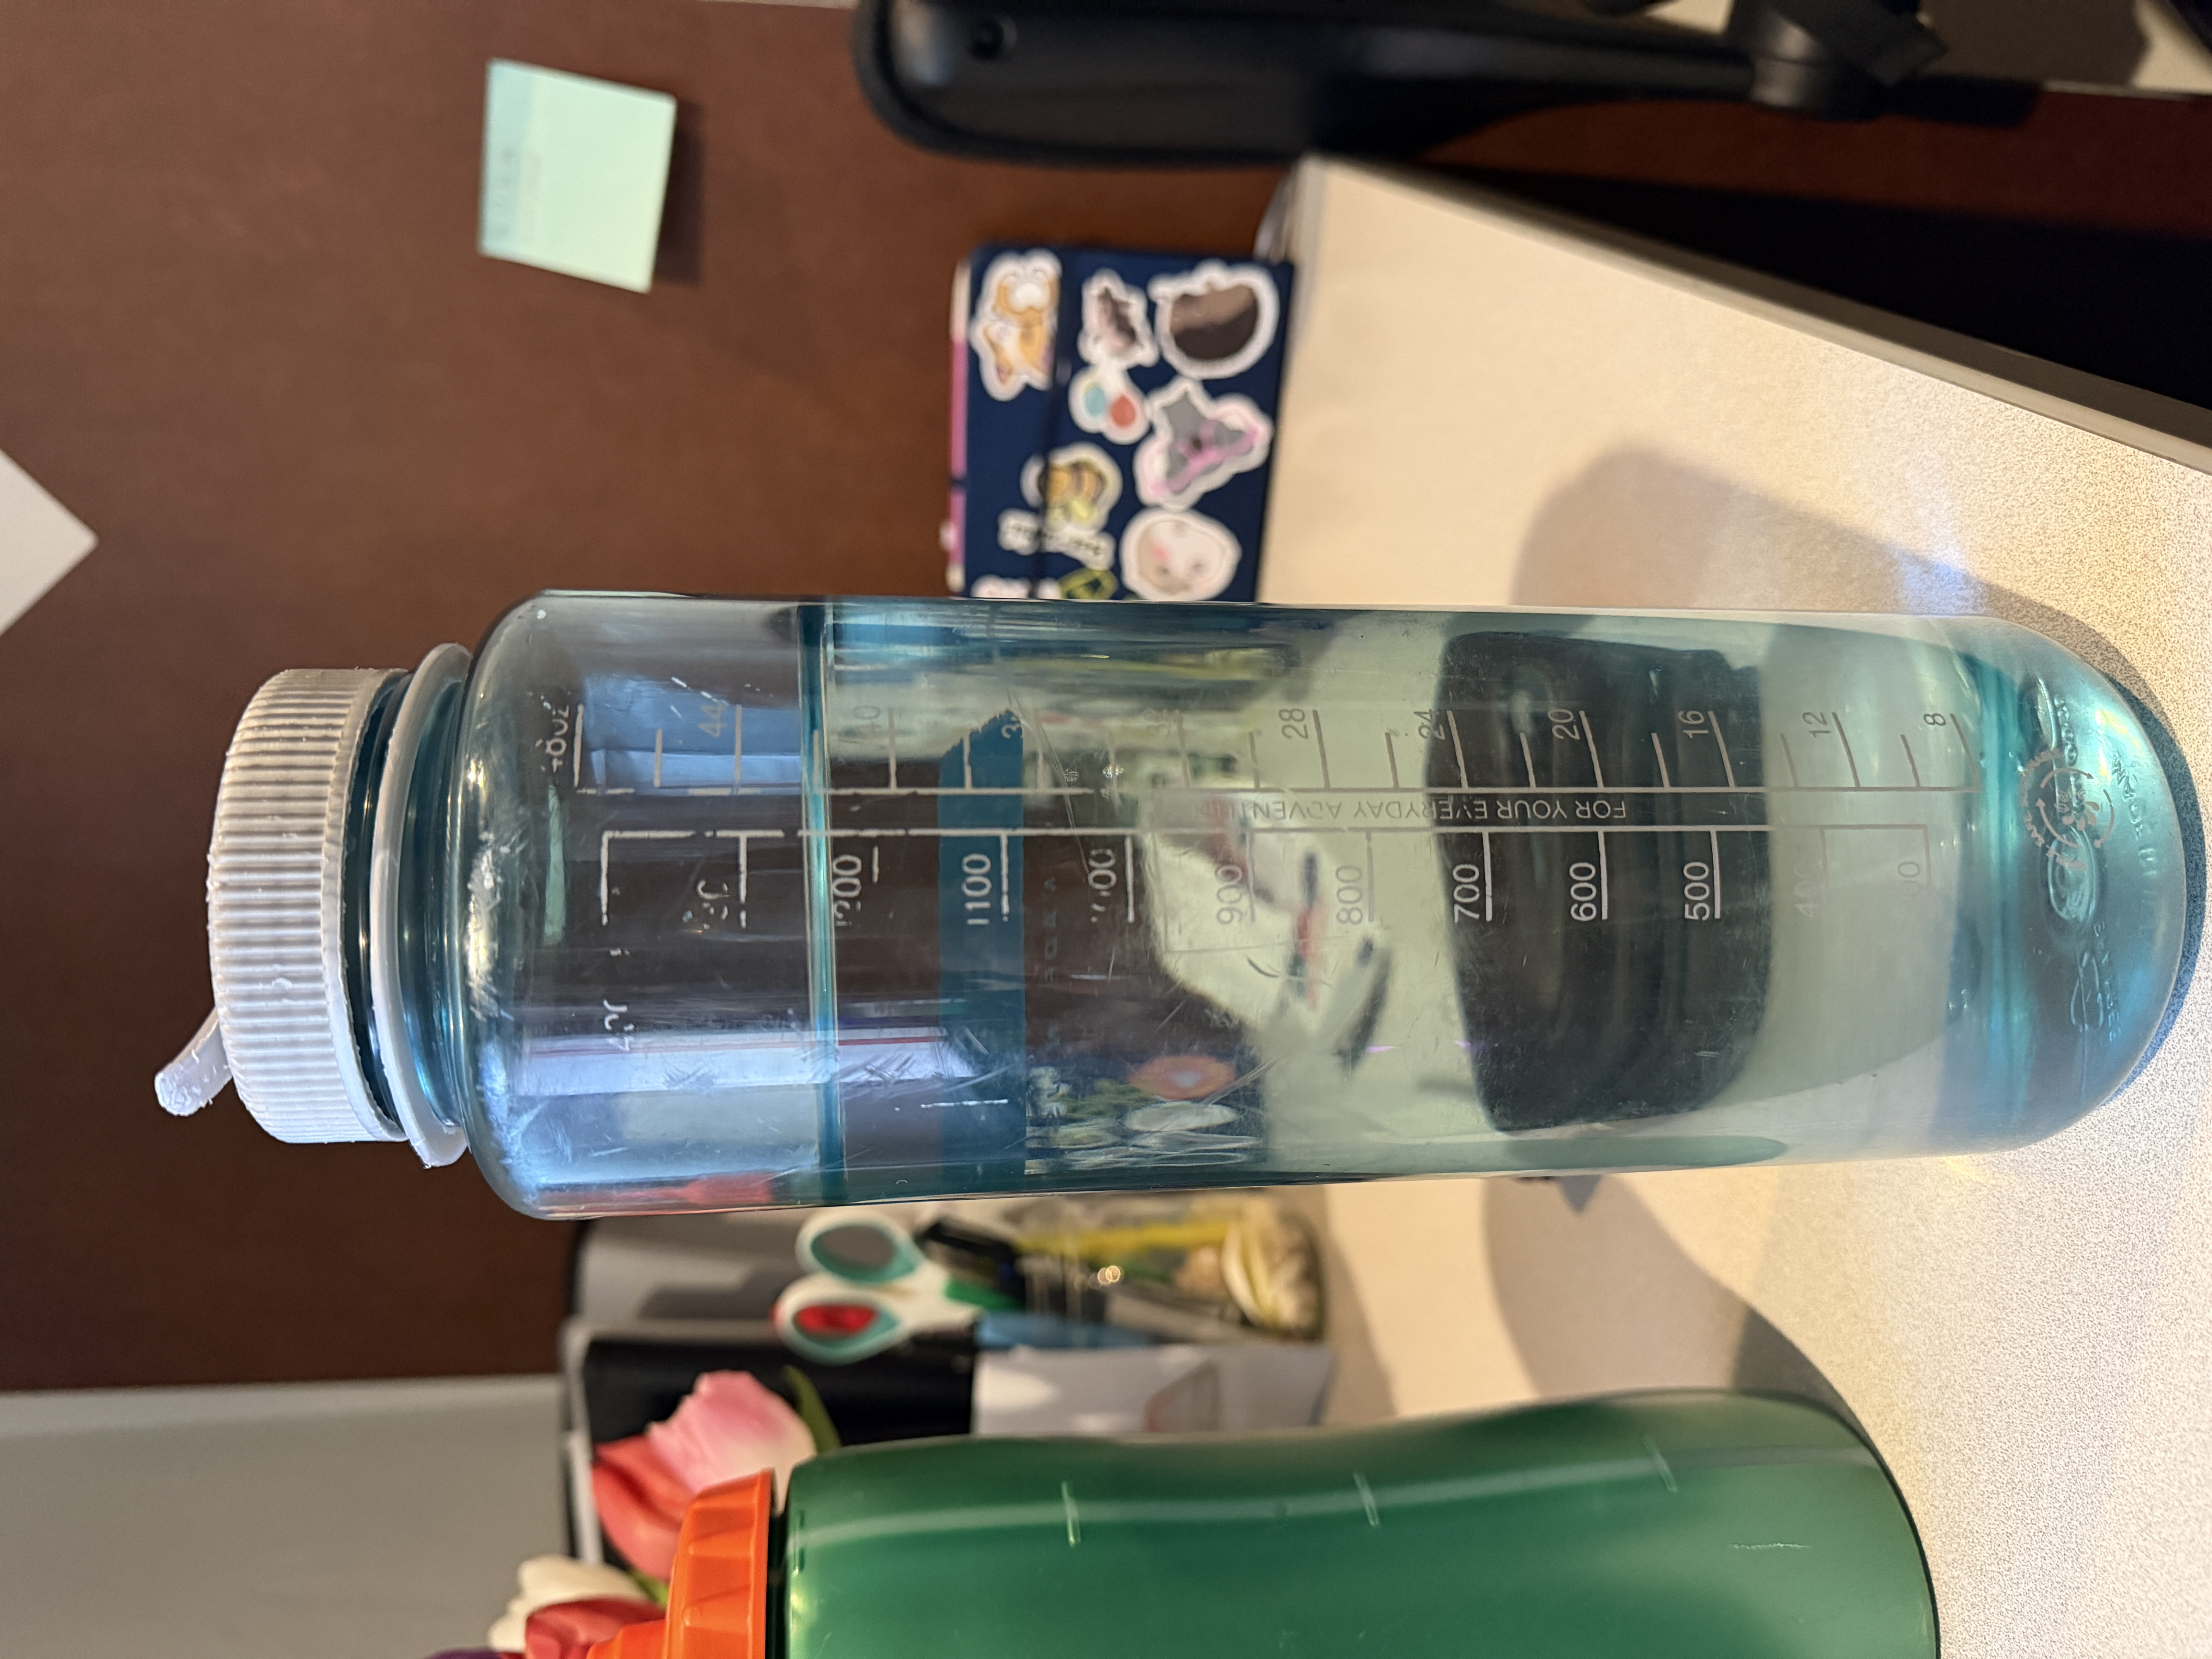
\includegraphics[width=0.45\textwidth,angle=-90]{images/water-level-visible-through-plastic.JPG}
\caption{Water level visible through transparent body.}
\end{figure}

The Brita filter also constrains flow speed and introduces additional alignment requirements.

\begin{figure}[H]
\centering
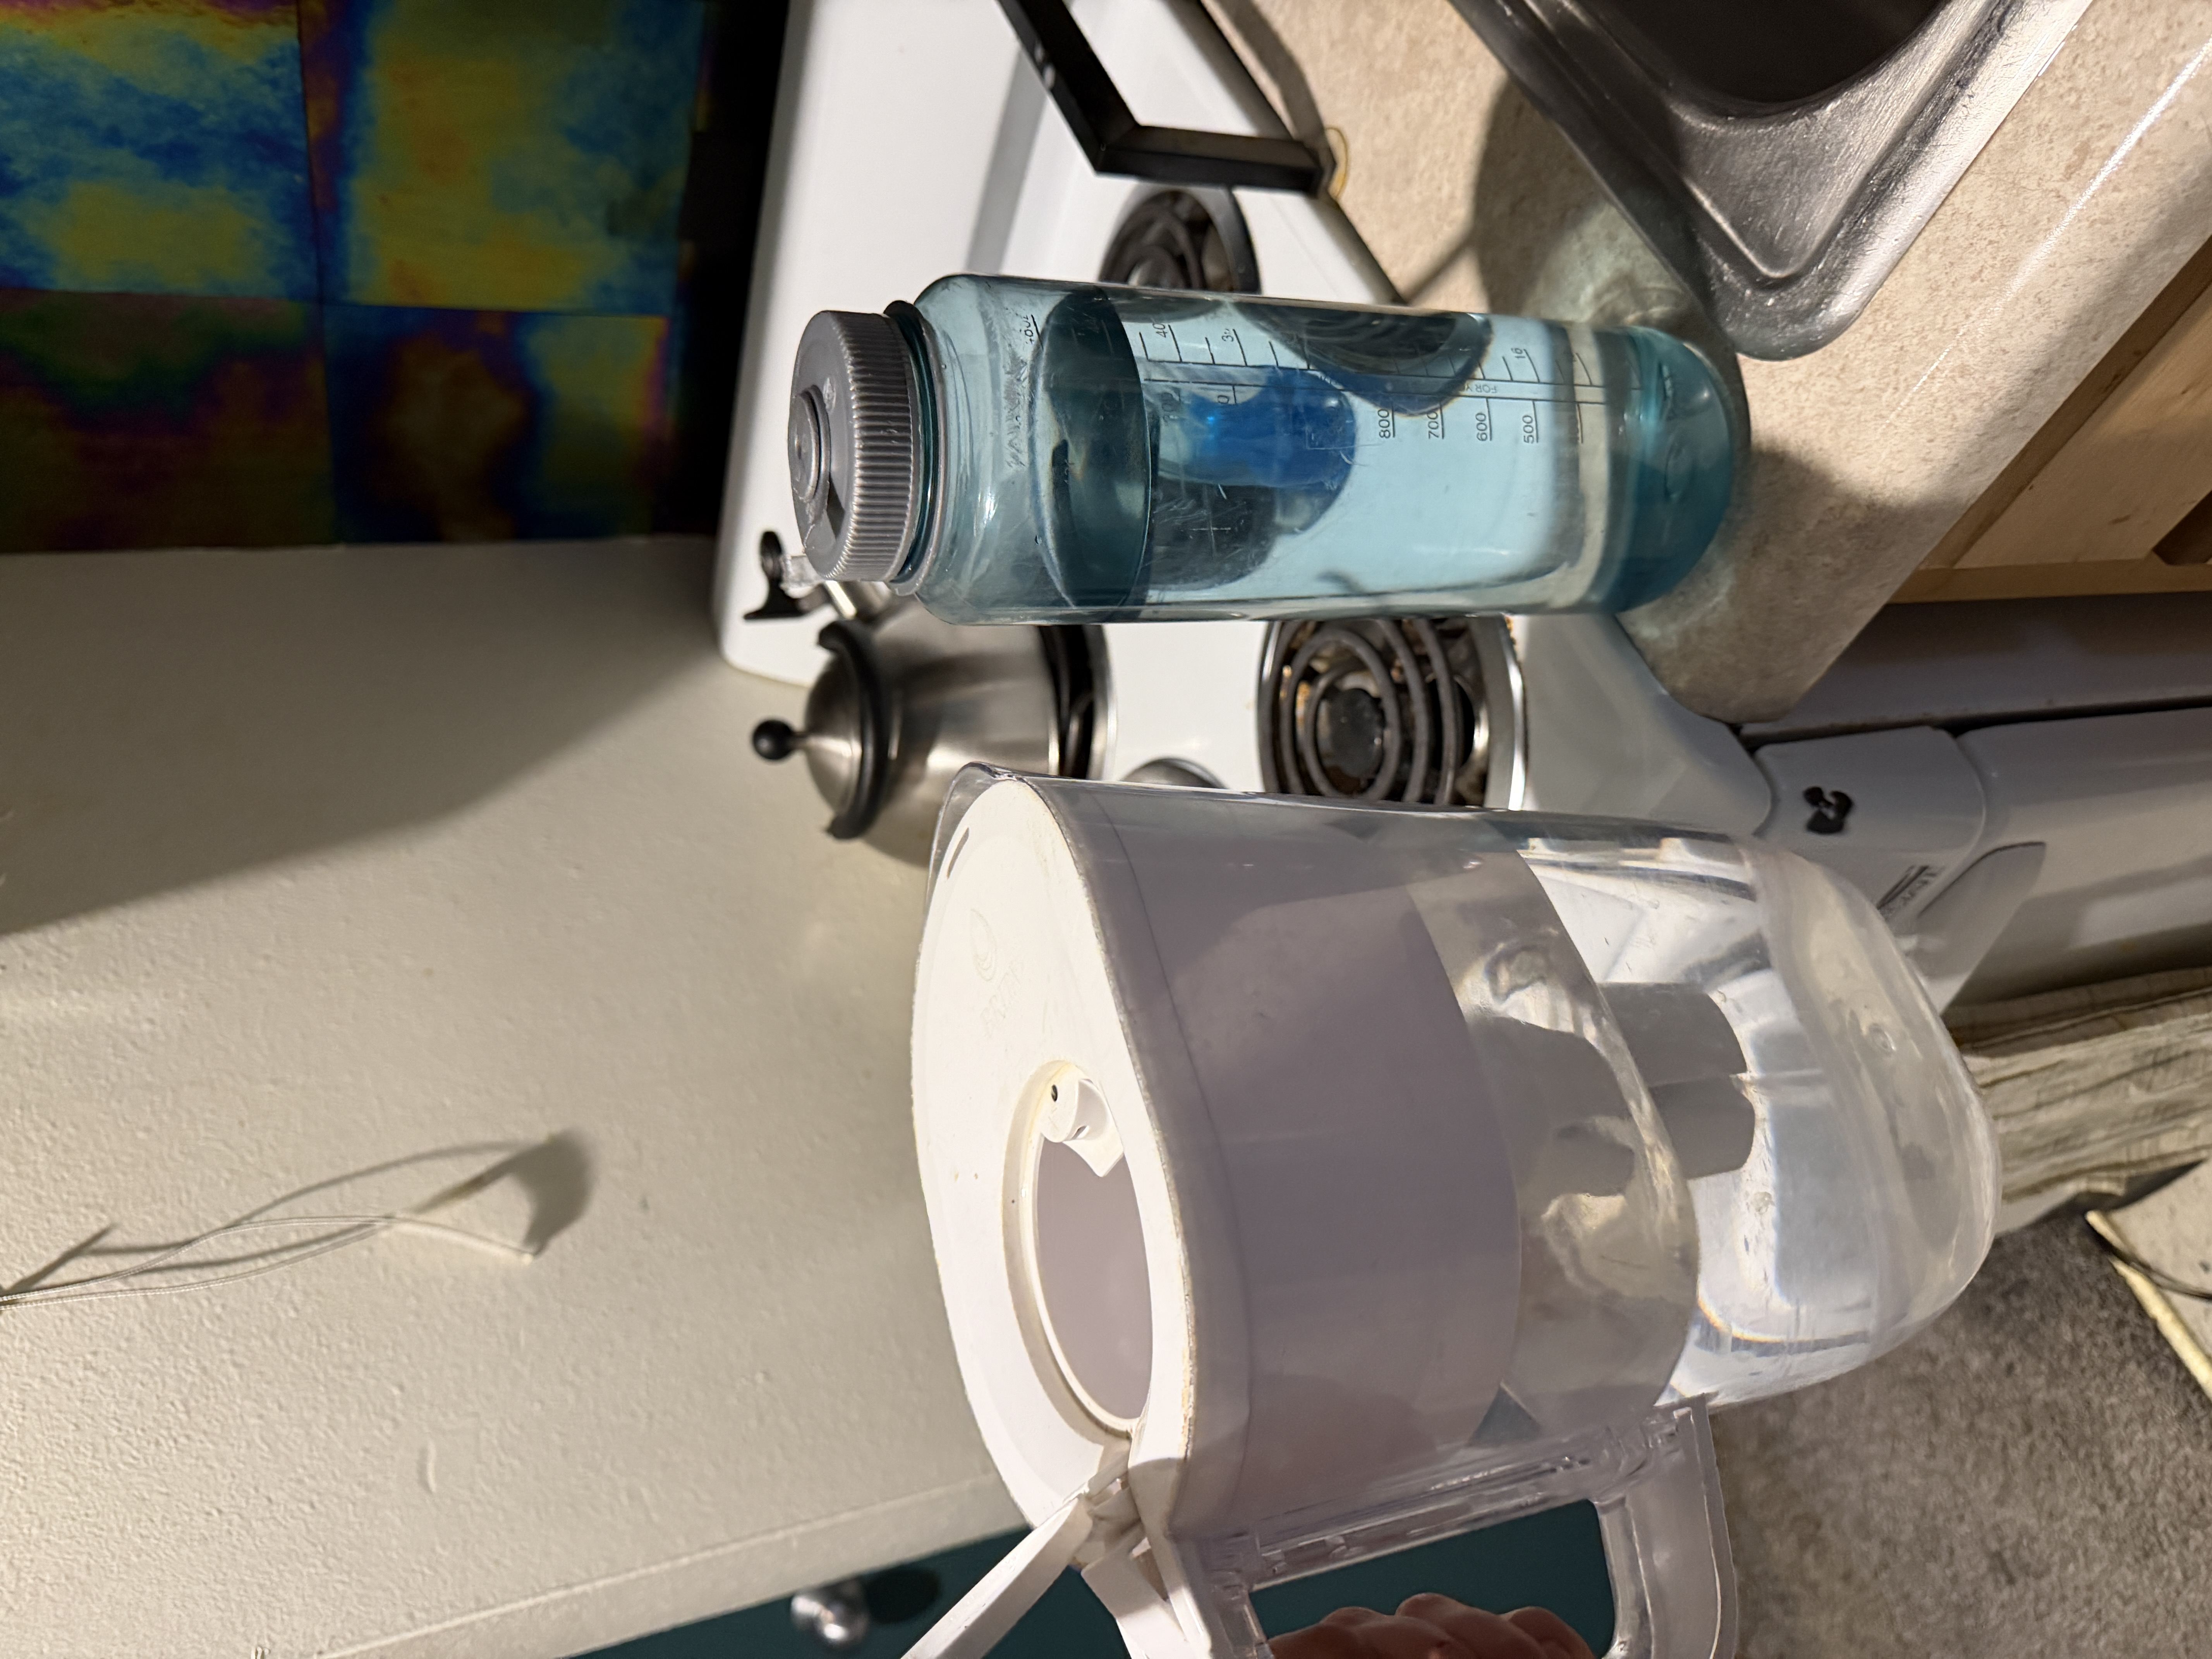
\includegraphics[width=0.45\textwidth,angle=-90]{images/brita-filter.JPG}
\caption{Brita filter used prior to transfer.}
\end{figure}

\subsection*{Step 3: Closing the Lid}

The lid must be aligned with internal threads before tightening. Misalignment prevents successful closure.

\begin{figure}[H]
\centering
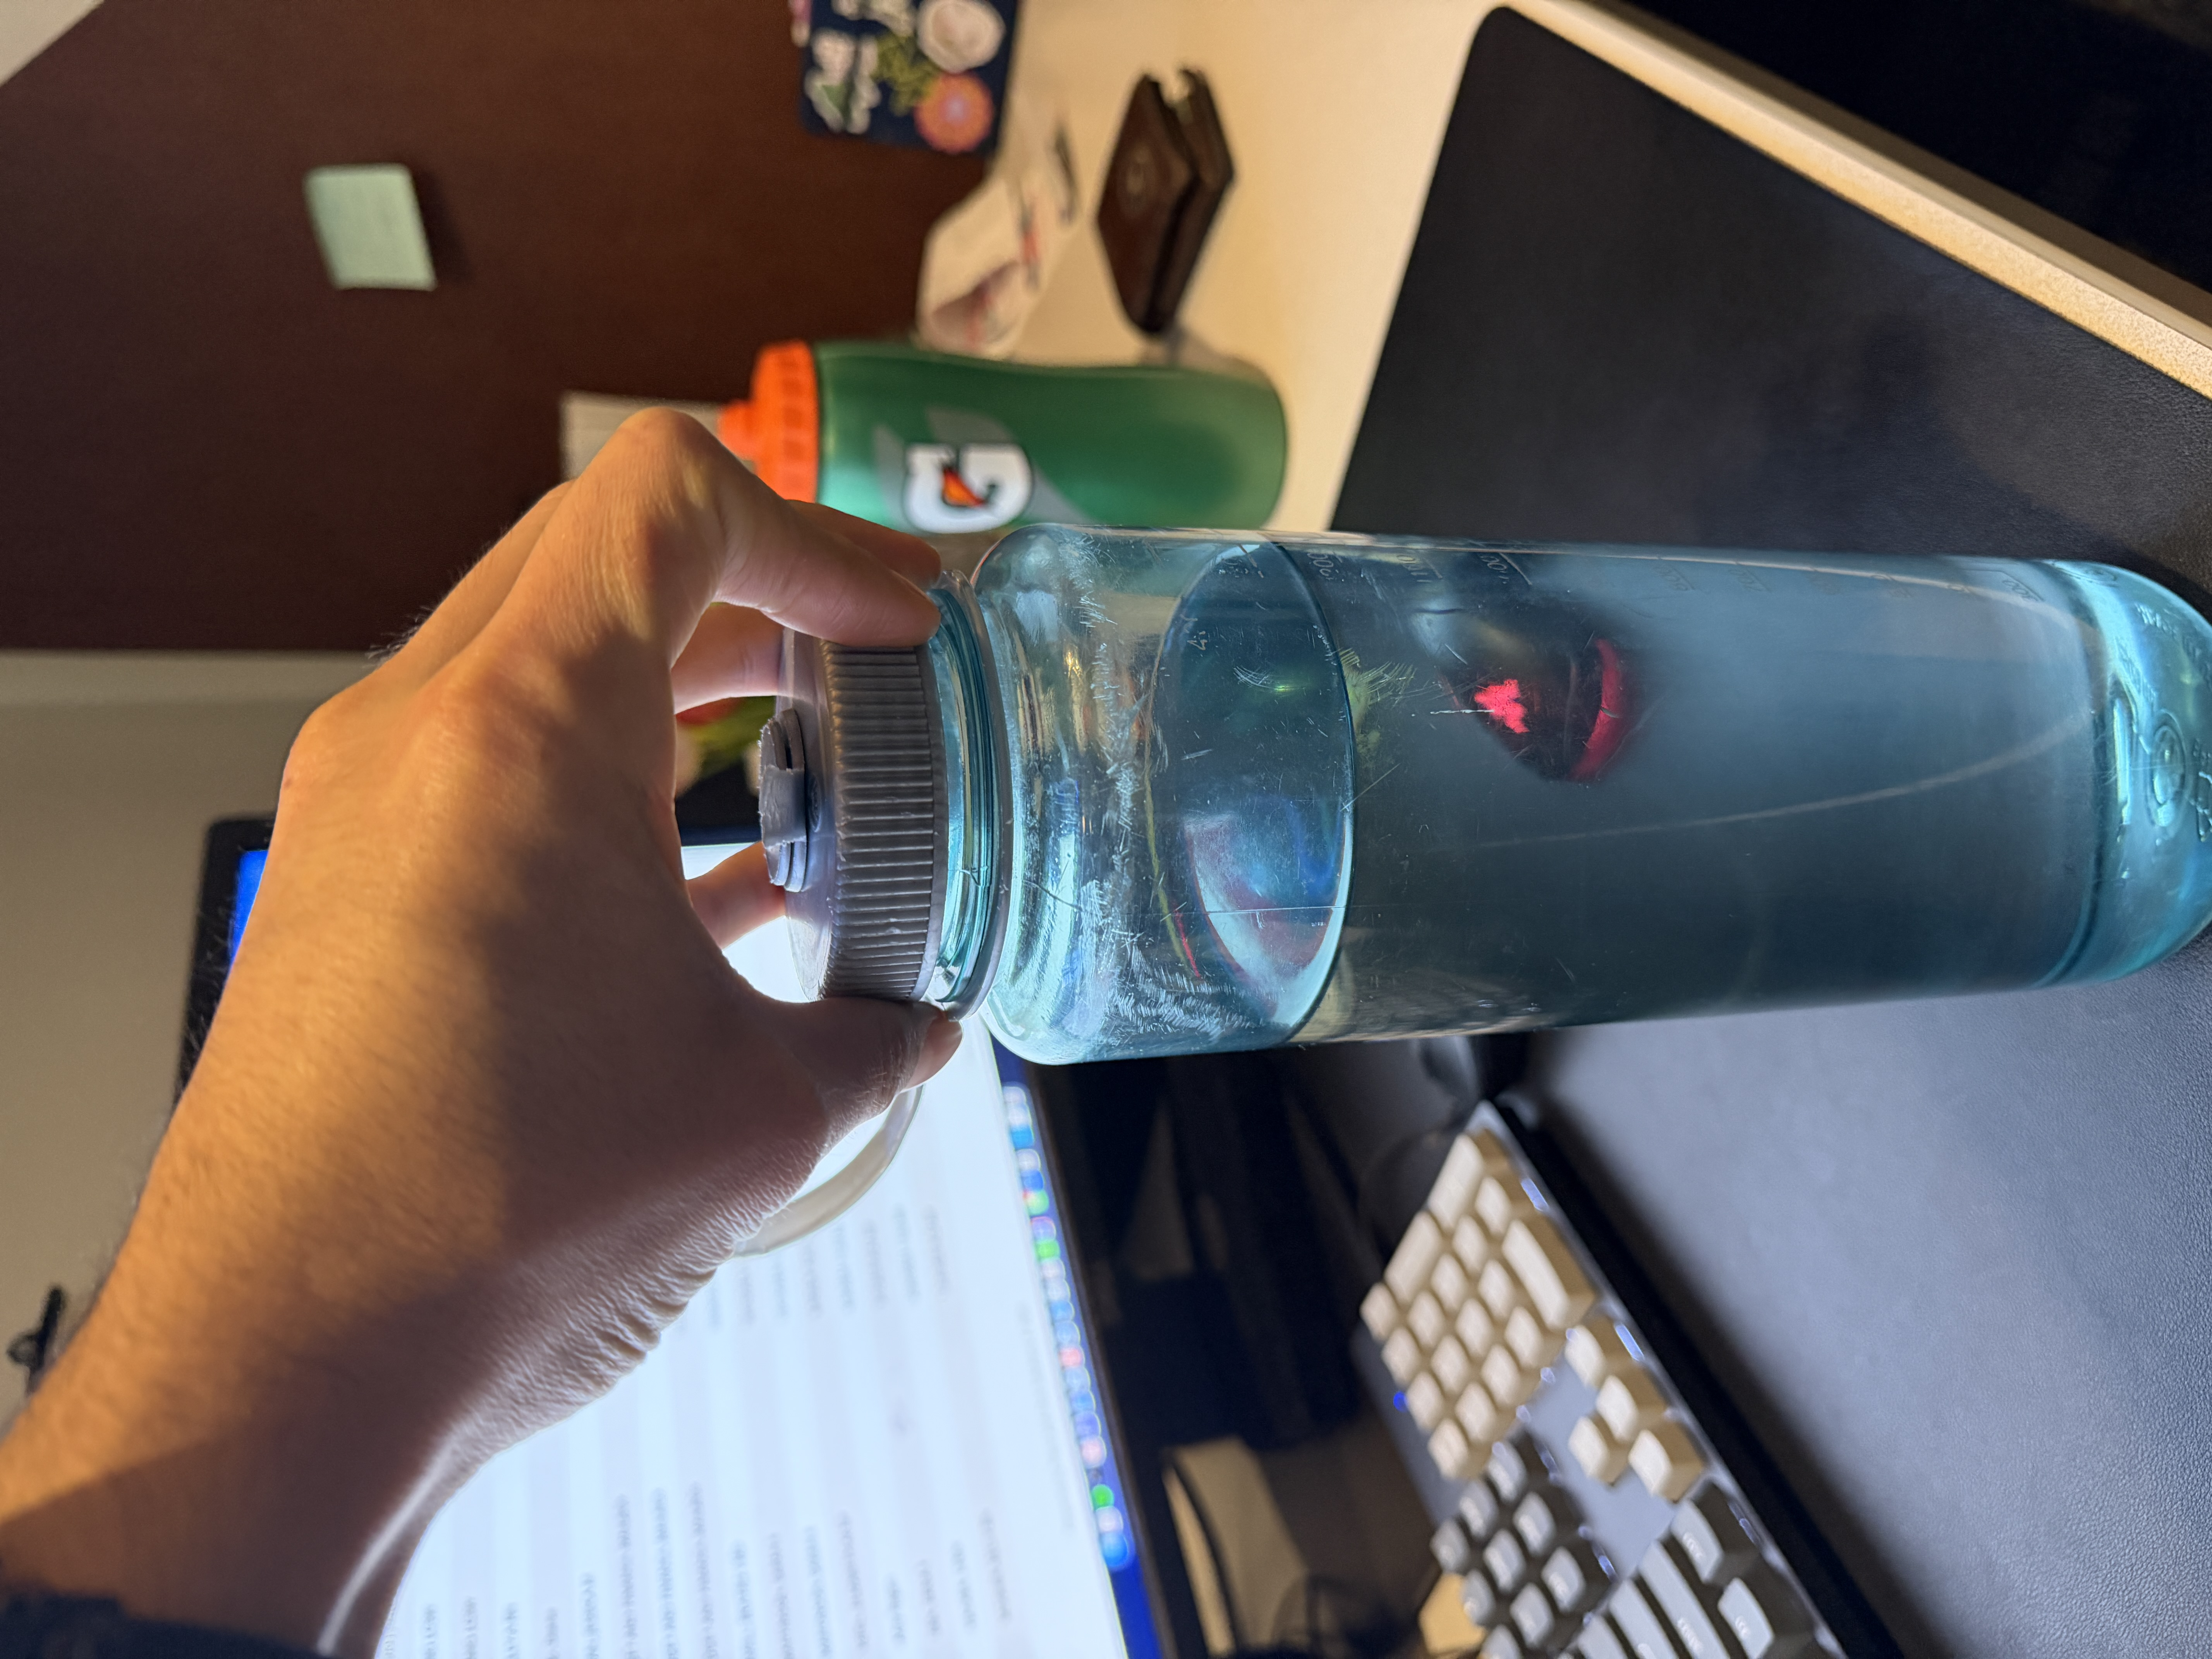
\includegraphics[width=0.45\textwidth,angle=-90]{images/screwing-lid-back-on.JPG}
\caption{Thread alignment and tightening.}
\end{figure}

The user relies heavily on tactile resistance to determine tightness. Under-tightening can cause dripping; over-tightening makes future opening difficult. This balance requires learned calibration.

\subsection*{Step 4: Transporting the Bottle}

Although the lid includes a loop attachment, the user does not rely on it due to structural weakness and residual droplets.

\begin{figure}[H]
\centering
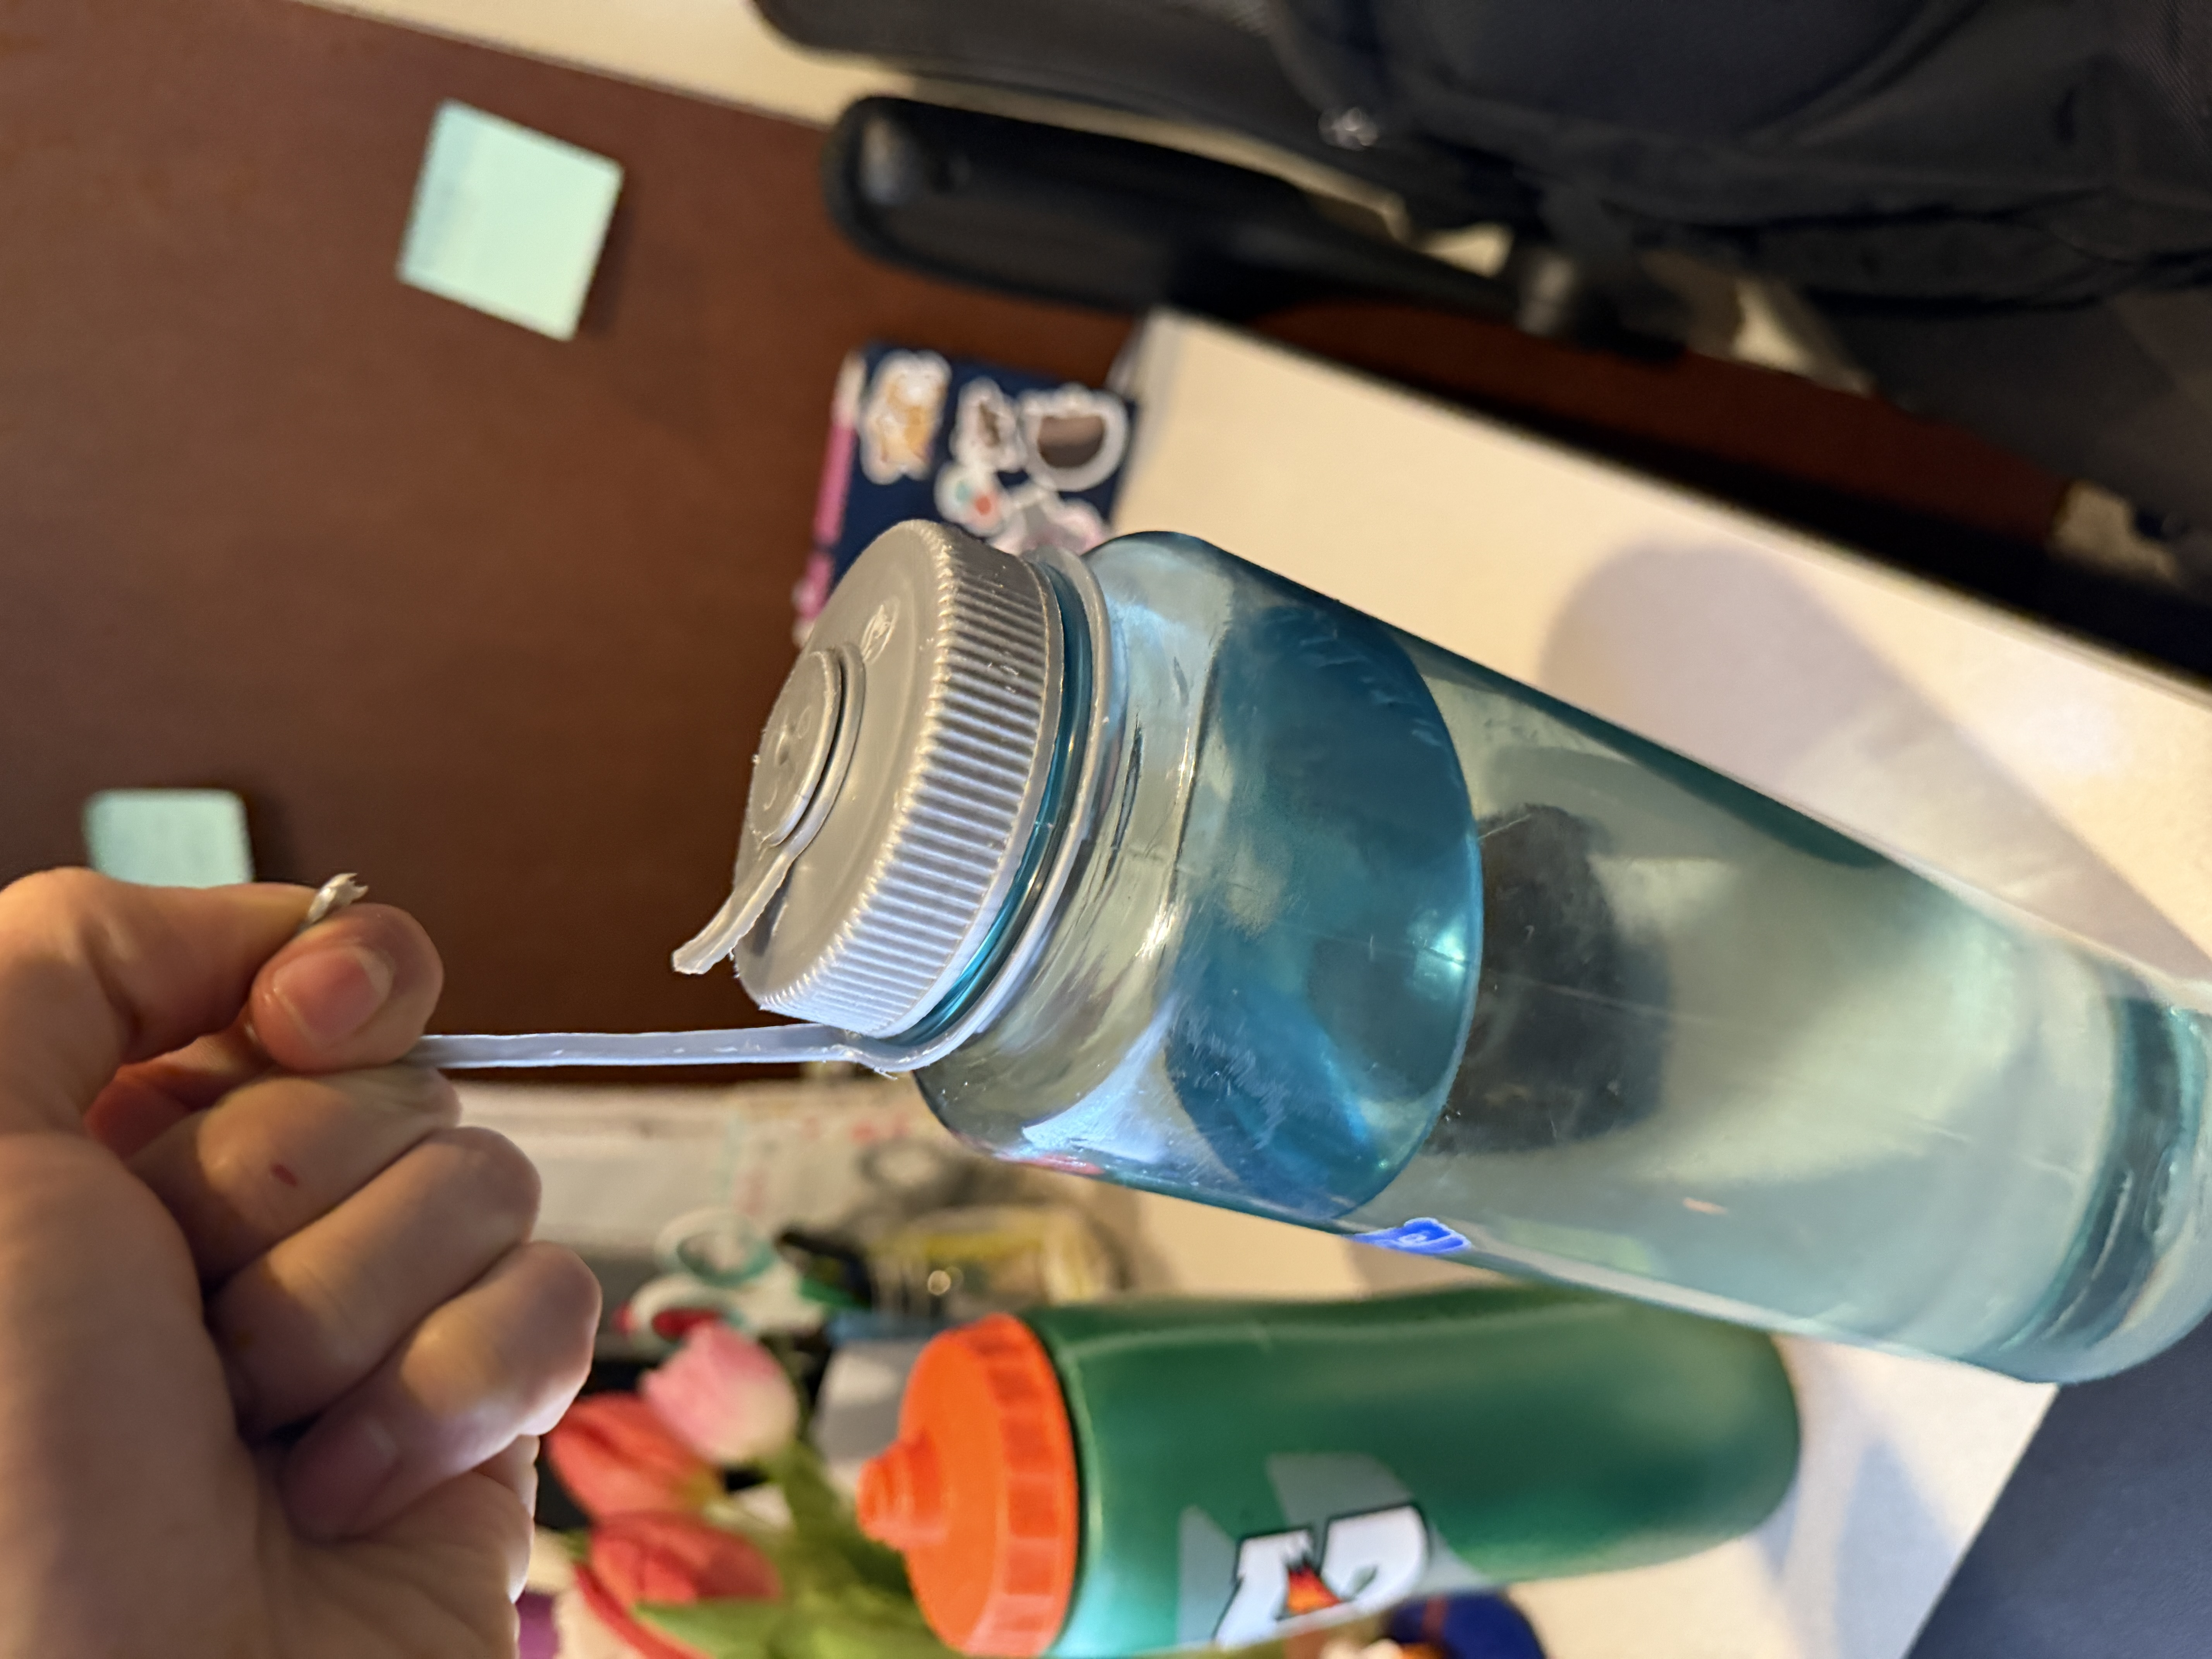
\includegraphics[width=0.45\textwidth,angle=-90]{images/carrying-broken-loop.JPG}
\caption{Loop attachment under stress.}
\end{figure}

Instead, the bottle is often carried against the body (``football carry'').

\begin{figure}[H]
\centering
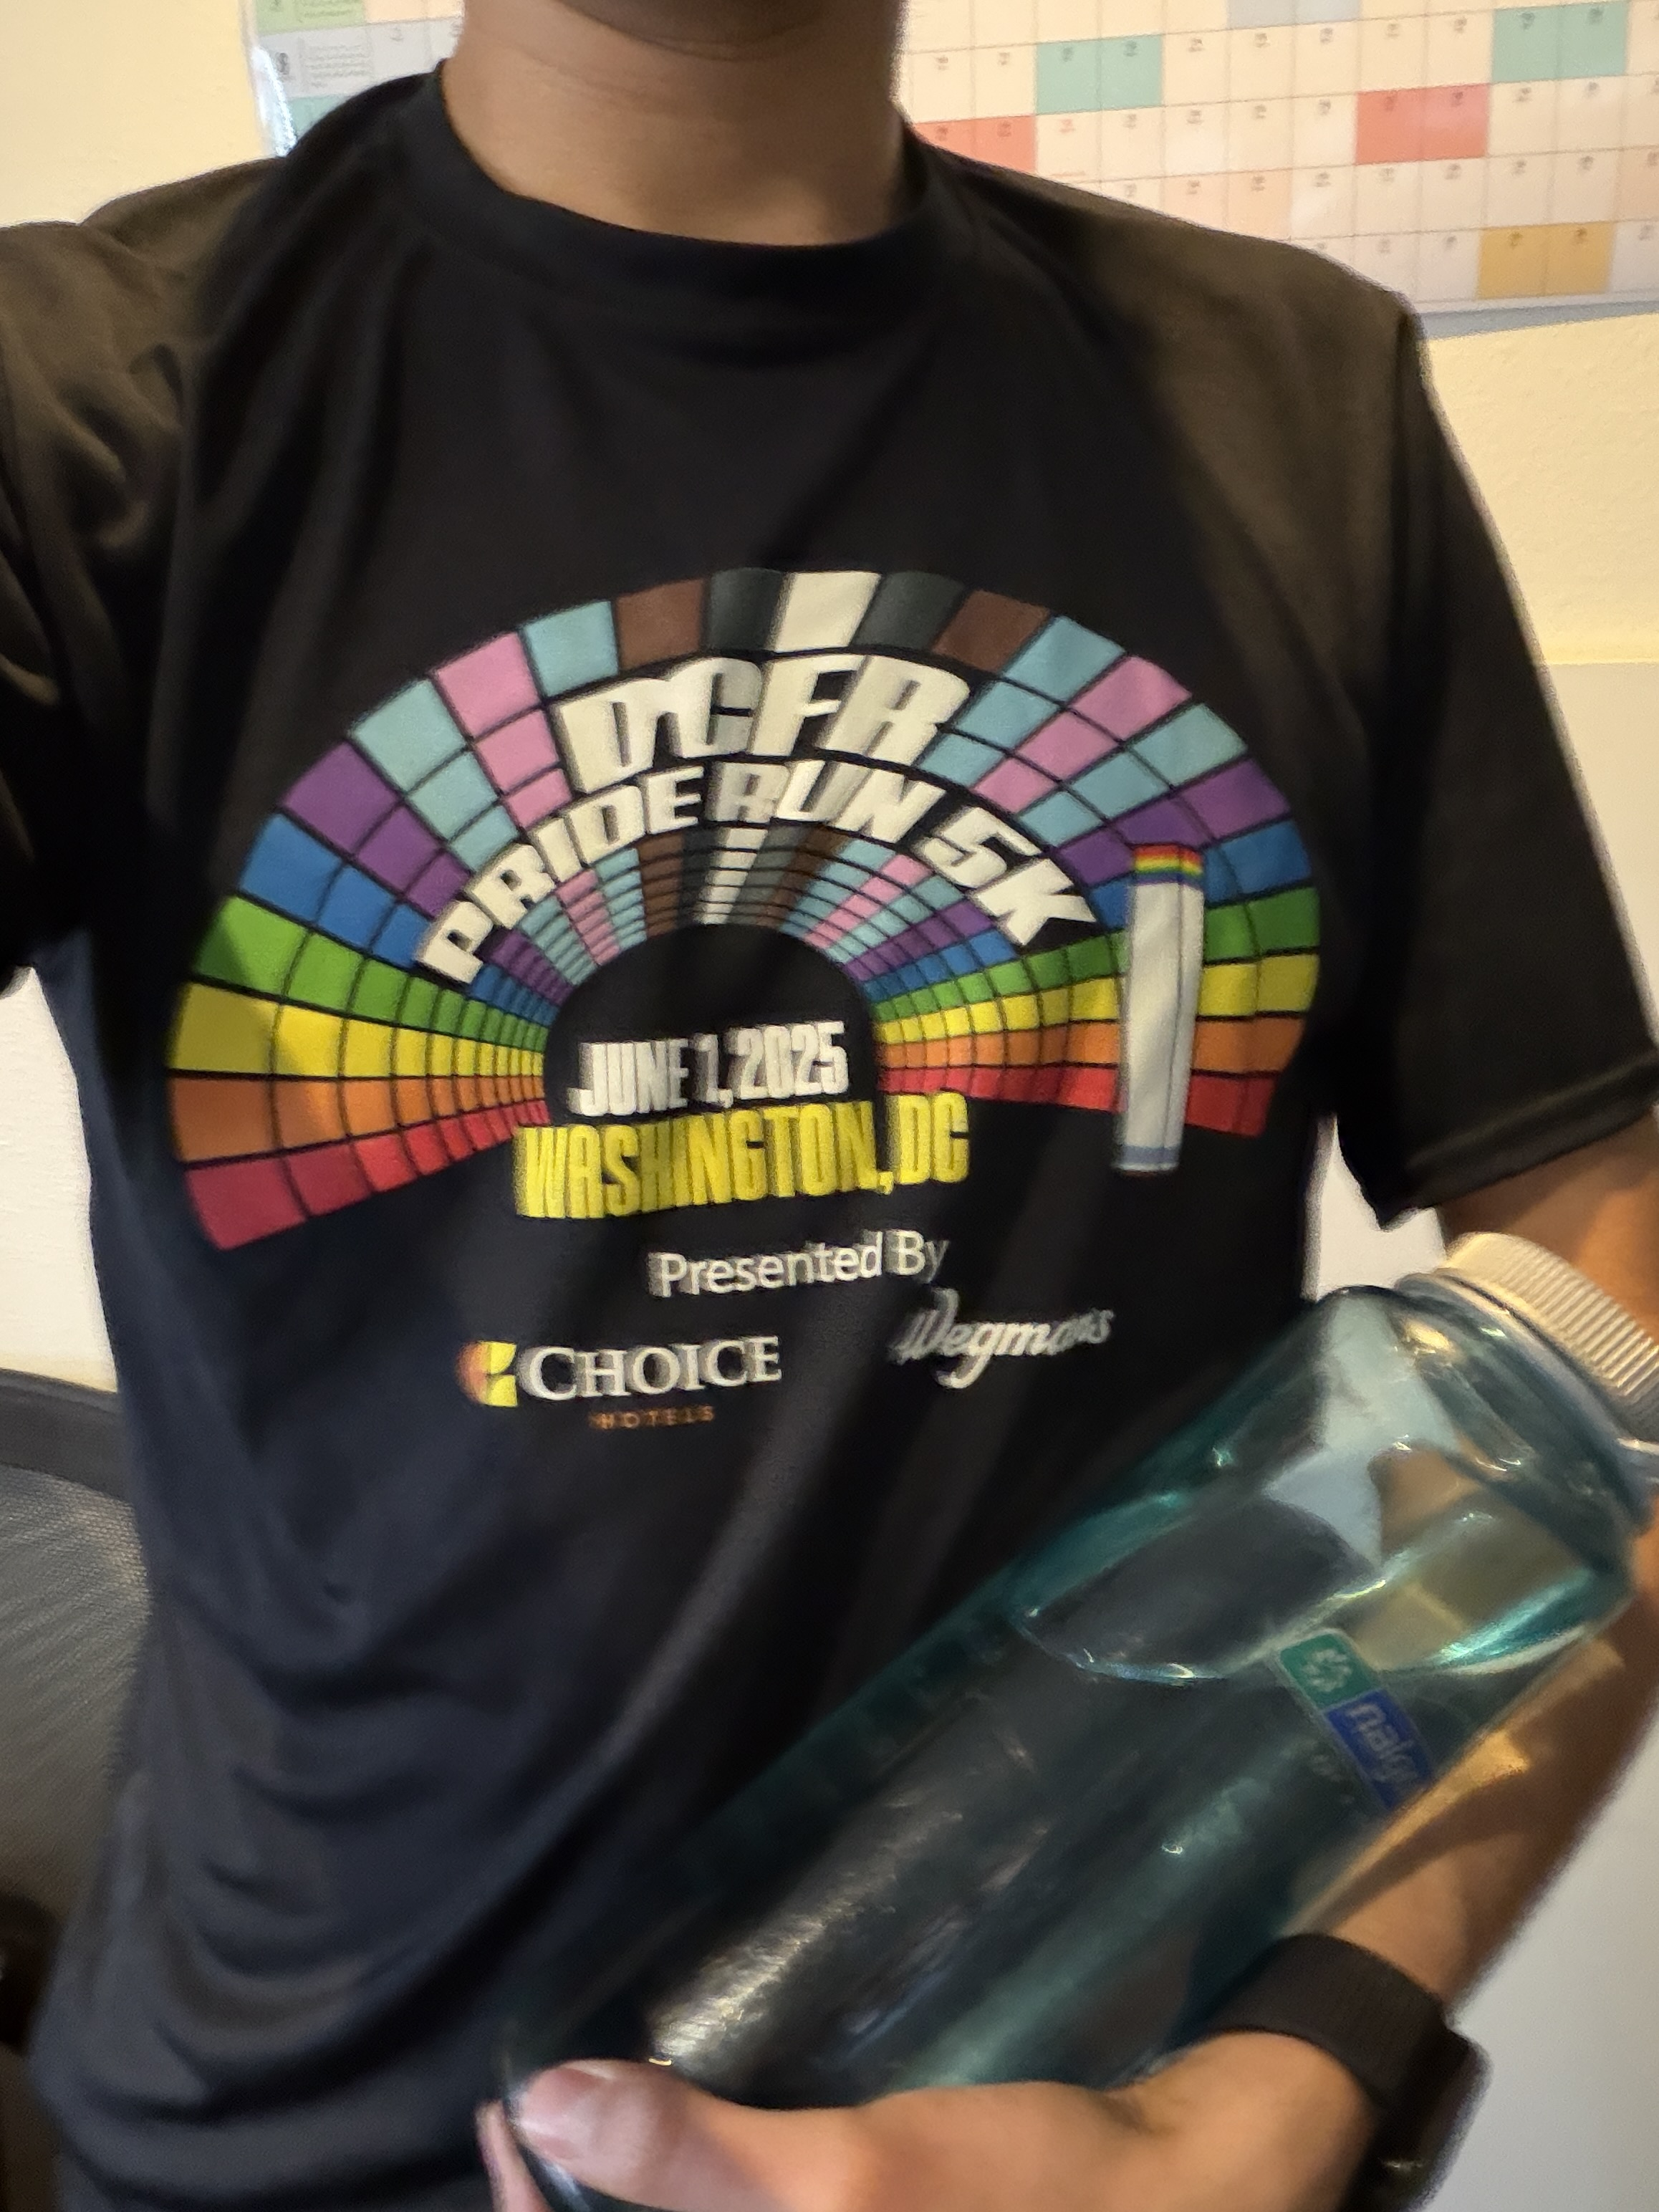
\includegraphics[width=0.45\textwidth,angle=-90]{images/football-carry.JPG}
\caption{Alternative carrying strategy.}
\end{figure}


\section*{Affordances}

The threaded lid affords rotational twisting in order to open and close the bottle. This affordance is supported by the cylindrical form and the ridged texture that suggests grip and torque application. The transparent plastic body affords visual monitoring of internal state, allowing the user to see the water level rise during filling and verify whether the bottle is empty or full without additional tools. The attached loop also affords carrying, although in practice this affordance is limited by its structural weakness and the presence of residual water droplets.

\section*{Signifiers}

The ridged texture on the lid acts as a signifier of grip and rotational movement, visually and tactually indicating that the lid should be twisted rather than pulled. The visible threading on both the bottle neck and the lid signifies a screw-based attachment mechanism, guiding the user toward alignment before tightening. Measurement markings along the side of the bottle serve as signifiers of volume, communicating how much liquid the container can hold and enabling rough tracking of consumption.

\section*{Constraints}

The internal thread design constrains how the lid can be attached, requiring proper alignment before tightening is possible. If misaligned, the lid resists closure, preventing improper sealing. The large diameter of the bottle constrains where it can be placed, limiting compatibility with smaller cup holders and certain carrying methods. Additionally, the need to balance tightness constrains user behavior: insufficient tightening leads to dripping, while over-tightening makes future opening difficult.

\section*{Feedback}

The system provides tactile feedback in the form of increasing resistance while tightening the lid, signaling when the seal is becoming secure. During filling, visual feedback is provided through the rising water line and visible bubbles, while auditory feedback changes as the echo inside the bottle diminishes when air space decreases. Weight increase offers additional haptic feedback once the bottle is lifted. Finally, dripping after closure serves as delayed negative feedback when the lid has not been tightened sufficiently.

\section*{Design Observations}

While the 48oz capacity supports hydration goals, its size introduces usability friction. Judging proper tightness requires experience, and residual droplets around the loop create minor but recurring inconvenience. The system demonstrates how even simple objects require ongoing cognitive calibration between force, sensory cues, and risk avoidance.

\end{document}
